%!TEX root = ../../../adrien_gomar_phd.tex

The first function to be tested with the convection model problem
is a sum of sine functions, the same used in the previous
section in Eq.~\eqref{eq:sum_sin}:
\begin{equation}
    u_0(t) = \cos(\omega t) + \sin(2 \omega t) +
    \cos(3 \omega t) + \sin(4 \omega t) + \cos(5 \omega t).
    \label{eq:sum_injected_fct}
\end{equation}
Harmonic balance computations are run with $1$ to $10$ harmonics.
For one computation, the results are presented 
using three sub-figures. Each 
sub-figure represents the spatial evolution of the velocity $u$
at three instants: $t=0$, $t=T/3$ and
$t=2T/3$. 
To produce these figures, a temporal interpolation is performed.
To do so, the frequency content of the harmonic balance result is used
together with an inverse Fourier transform on the following time-vector
$[0, T/3, 2T/3]$.

These sub-figures allows to underline
the spatial evolution for specified time instants, showing
the complex spatio-temporal structure of the results. 
As the largest period of
the temporal phenomenon is set to fit the domain size
(recall Eq.~\eqref{eq:time_spatial_correspondence}), only one
pattern of the function is spatially seen.

\begin{figure}[htbp]
  \centering
  \subfigure[$N=1$ computation]{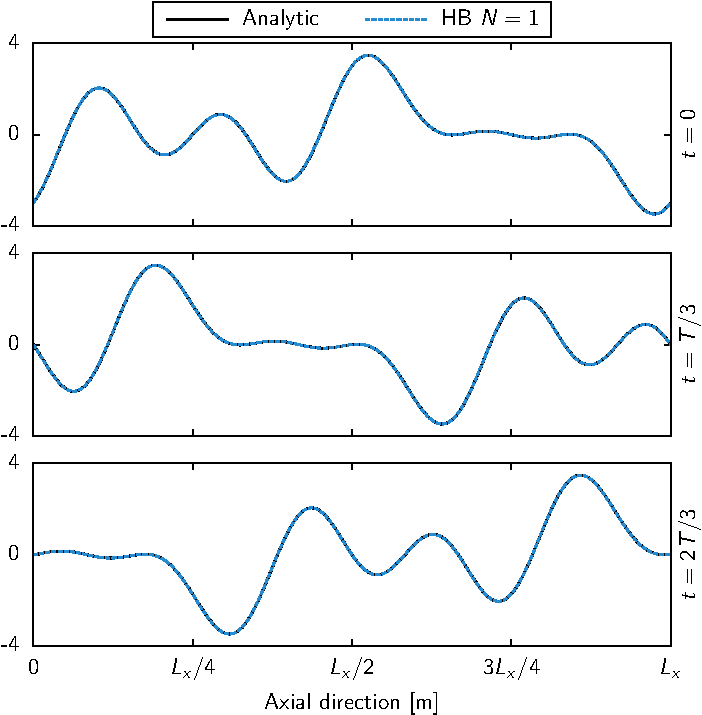
\includegraphics[width=.35\textwidth]{convection_sin_N1.pdf}}
  \subfigure[$N=2$ computation]{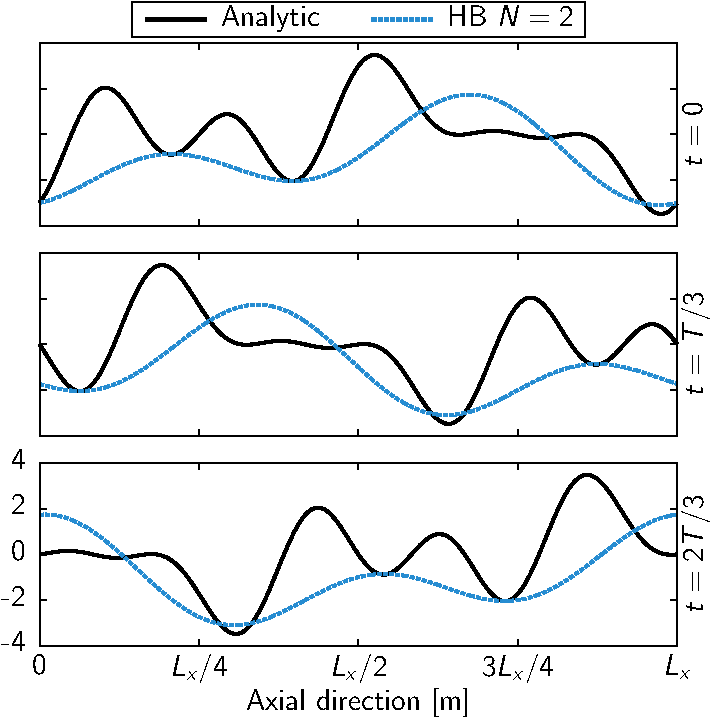
\includegraphics[width=.35\textwidth]{convection_sin_N2.pdf}}
  \subfigure[$N=3$ computation]{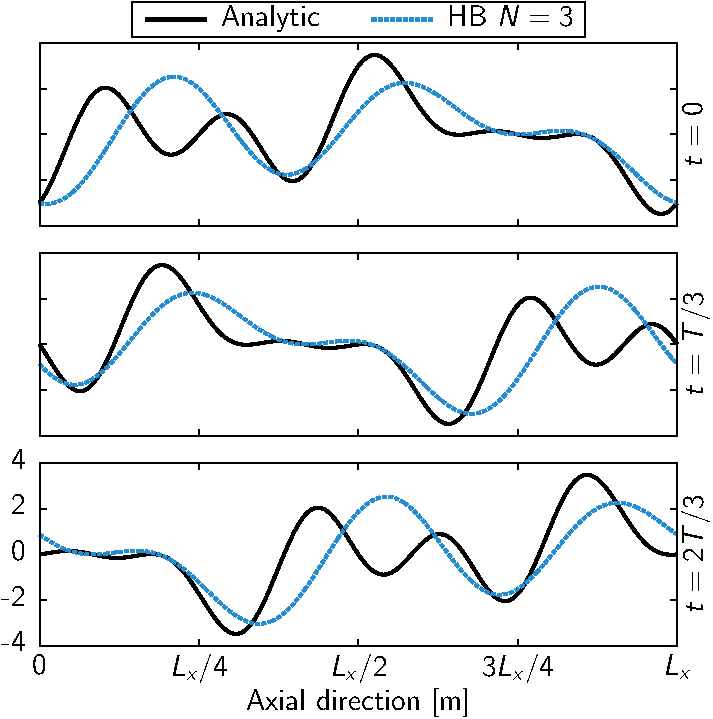
\includegraphics[width=.35\textwidth]{convection_sin_N3.pdf}}
  \subfigure[$N=4$ computation]{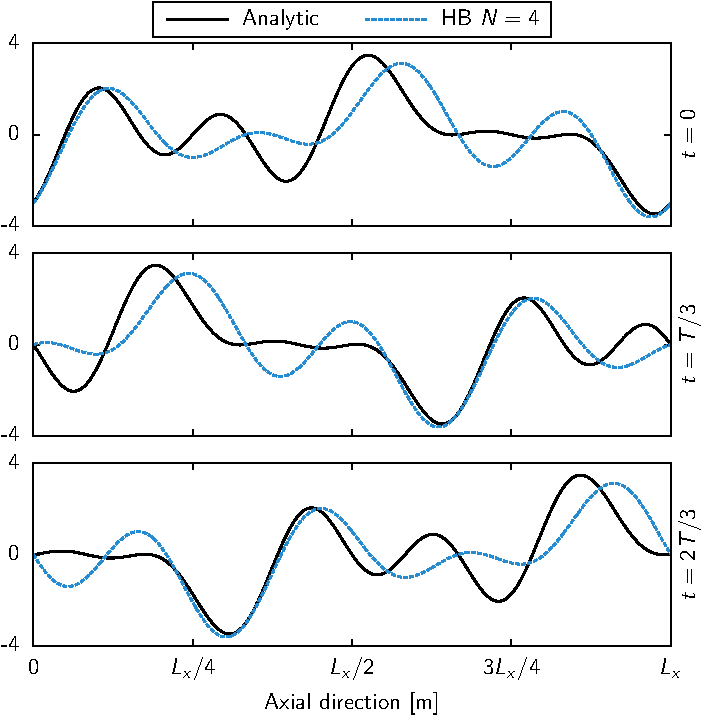
\includegraphics[width=.35\textwidth]{convection_sin_N4.pdf}}
  \subfigure[$N=5$ computation]{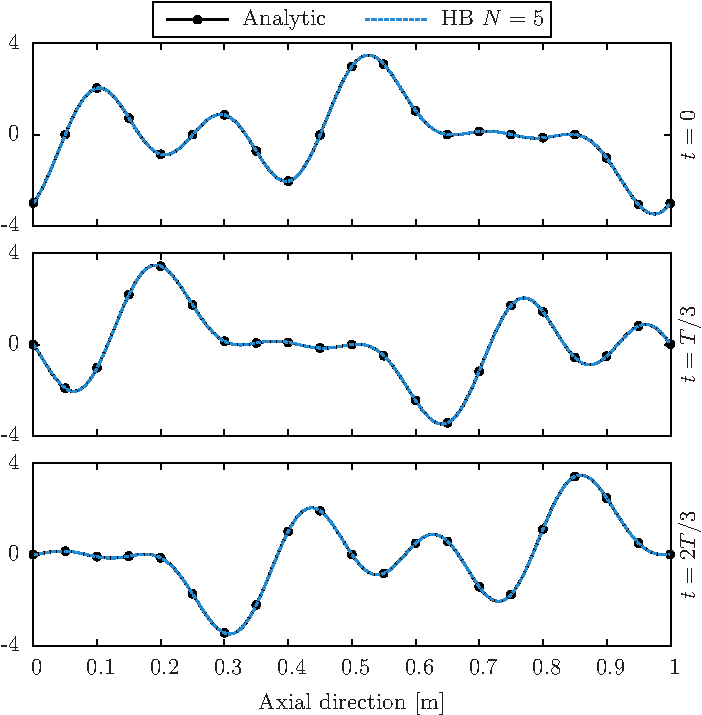
\includegraphics[width=.35\textwidth]{convection_sin_N5.pdf}}
  \subfigure[$N=6$ computation]{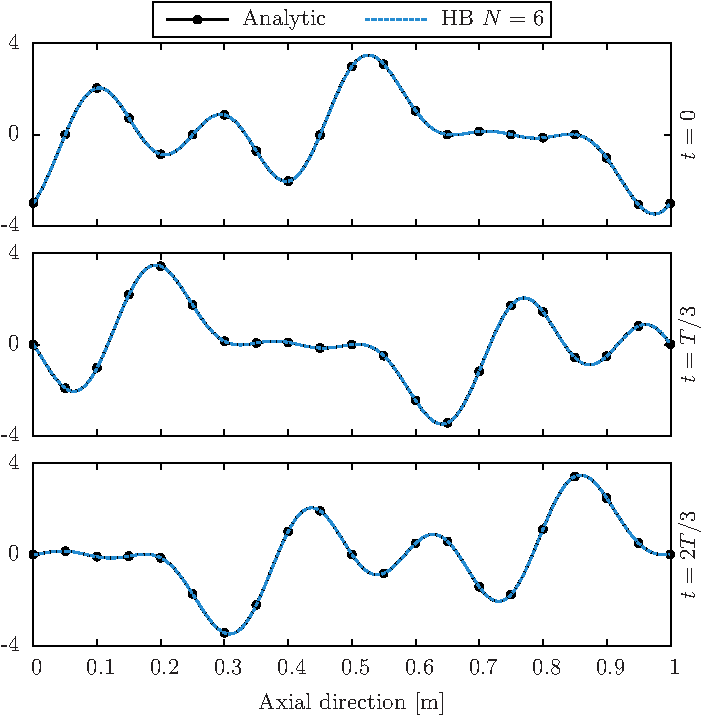
\includegraphics[width=.35\textwidth]{convection_sin_N6.pdf}}
  \caption{Harmonic balance results for 
  an injected sum of sine functions.}
  \label{fig:inj_sine_results}
\end{figure}

Figure~\ref{fig:inj_sine_results} depicts the harmonic balance
computations from $1$ to $6$ harmonics. Only those are shown
as they are sufficient to highlight the main qualitative effects. However,
all the calculation results will be used latter-on to quantitatively
analyze the convergence error.
The analytical solution is
drawn for comparison. 
It can be seen that, the more harmonics in the
computations, the closer the results to the analytical solution.
The shape of the solution 
is constantly improved until it reaches the frequency content
of the injected signal.
When it is the case
(here $5$ harmonics, see Eq.~\eqref{eq:sum_injected_fct}),
the results of the harmonic balance computation are
superimposed with the analytical solution. Adding
more harmonics in the computation does not improve
the solution. This effect was already seen on the previous section
in Fig.~\ref{fig:hb_operator_sample}.

The $\mathcal{L}_2$-norm of the error as described
in Eq.~\eqref{eq:l2_norm} is computed for each harmonic balance
computations to get the convergence rate of these calculations. It is
shown in Fig.~\ref{fig:conv_sum_sine}. Two results are displayed:
one for the reference mesh ($2000$ grid points) and one for
a refined mesh ($4000$ grid points).
\begin{figure}[htbp]
  \centering
  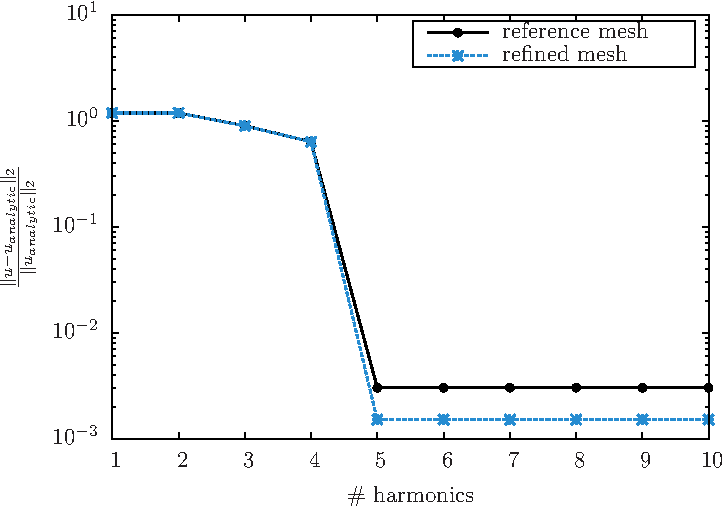
\includegraphics[width=.5\textwidth]{convection_sin_error.pdf}
  \caption{Convergence of the harmonic computations for an injected sum of sine functions.}
  \label{fig:conv_sum_sine}
\end{figure}
The convergence of the harmonic balance computations is slow  for
$N \leq 4$. However, when the number of harmonics composing
the injected function is reached ($N=5$), the error is minimum and computing
more harmonics does not change the error. 
The value of the plateau obtained 
after $N=5$ is representative of the error introduced by the spatial
discretization. In fact, refining the mesh changes this value
without modifying the error levels of the lower harmonics points.
Note that the error that is measured is the true residual, meaning
that the computation is compared to the analytical result.
This is why, the only way to have a zero machine value like in
Fig.~\ref{fig:hb_operator_error}, is to have an infinite number of grid points.

The convergence rate 
of Fourier-based methods is inherently linked to the spectrum of the
temporal phenomenon that one wants to capture.
To verify this, the temporal discrete Fourier transform
of the computational results is displayed against 
analytical results in Fig.~\ref{fig:dft_sin}.
\begin{figure}[htbp]
  \centering
  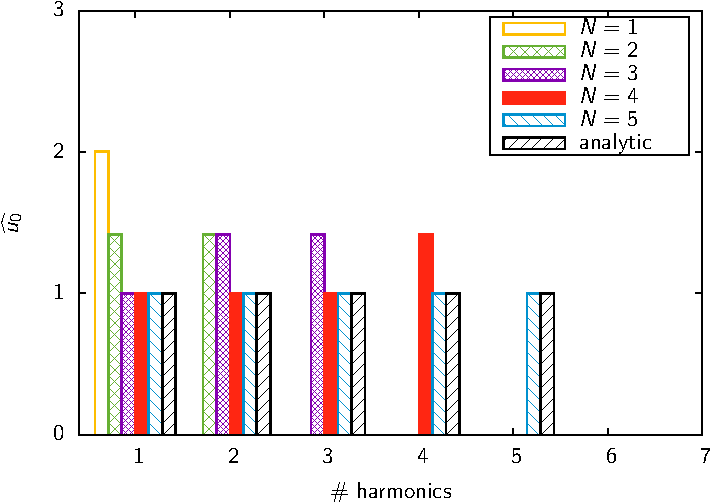
\includegraphics[width=.5\textwidth]{convection_sin_dft.pdf}
  \caption{Discrete Fourier transform of the computational
  results compared to the analytical one for an injected sum of sine
  functions.}
  \label{fig:dft_sin}
\end{figure}
When the number of harmonics grows in the spectral computations,
the Fourier transform gets closer to the analytical solution.
Albeit it reaches the whole frequency content, the computational
results are superimposed with the analytical ones. One can also
notice that meanwhile, the intermediate frequencies, as for 
instance the $N=3$ harmonics computation, almost retrieve 
the amplitudes that can not be captured by the harmonics that are
not computed. The threshold effect seen above for the convergence can be highlighted
here: when the number of harmonics composing the spectrum of the
computed signal is reached, the computational results are exact, compared
to the analytical ones. This is true since the signal that
one wants to capture is adapted to the current approach as Fourier-based methods
are designed to captured periodic fields by decomposing them
using a sum of sine functions. 

To further analyze the convergence of Fourier-based methods, a more
demanding function for harmonic balance approaches is computed: the
rectangular function.